\entry{2026-10-18}{Priority 1: cost and accuracy against bank width $r$ and mesh $N$ (2D, plus 3D kernels)}

Lane \texttt{2026-10-17-jcp-p1-scaling}, last commit \texttt{5b782026b}, mirror \texttt{3b589dad5}. Eleven jobs (A100/H200, all \texttt{jax\_backend=gpu}), 1.91 of the 20 GPU-h cap; nothing deferred. Design restated by the coordinator from plan v4 and Codex-audited (4 rounds) before launch; lane audits: design 5 rounds, code 4, jobs 5, results/report 4, all clean at the end. Numbers quoted from the generated \path{report.md}. Errors are against E0 $R_{ST}$ (conditional Richardson $\varepsilon_{\rm ref}$).

\begin{itemize}
\item \textbf{Solve cost is mesh-independent (H-cost-N): pass, 8/8 configurations} ($r=128,256,384$; BE and CN-R; $256^2$, $1024^2$, $4096^2$). Max/min solve time over meshes 1.01--1.02, every 95\,\% interval $\le 1.04$ (bar 1.25). Coordinator recheck from raw timings: 1.0085--1.016.
\item \textbf{Accuracy is mesh-independent (H-acc-N): pass, 8/8.} Every case within its margin (38 cases at $256^2$, 16 at $4096^2$). R128 CN-R shows a small detectable trend ($p=0.0063$), so ``pass'' there means practical equivalence within the margin.
\item \textbf{Accuracy improves with $r$ (H-acc-r):} 128$\to$256$\to$384 improves at every mesh and for both schemes (majority of resolved cases). 384$\to$512 at $1024^2$ does \emph{not} improve (BE 4 better / 16 worse / 18 tied; CN-R 6/22/10): the known regression is reproduced.
\item \textbf{Kernel cost against $r$ (H-cost-r): 7 of 8 component fits fail} their declared operation-count exponents. Cholesky grows like $r^{1.24}$ (2D) and $r^{1.03}$ (3D) instead of $r^3$; $J^\top J$ like $r^{1.92}$ / $r^{1.33}$ instead of $r^2$. At these sizes the GPU kernels are far from their asymptotic regime; this is a statement about measured cost, not about operation counts.
\item \textbf{Qualification:} all 22 rollout configurations pass Q1 (solver) and Q2 (quadrature). The archived combined-lane 1024$^2$ results reproduce to $\le 2.9\times10^{-15}$.
\item \textbf{P1g, the frozen mode list:} the 2D test-mode set differs only at $256^2$ (2 of 1536 modes swapped); at $4096^2$ it is the same set in another order. Freezing it moves trajectories by $5$--$9\times10^{-4}$ but errors by only 0.01--0.05 percentage points. Earlier cross-mesh claims compared slightly different test spaces at $256^2$; the conclusion does not change.
\end{itemize}
\begin{center}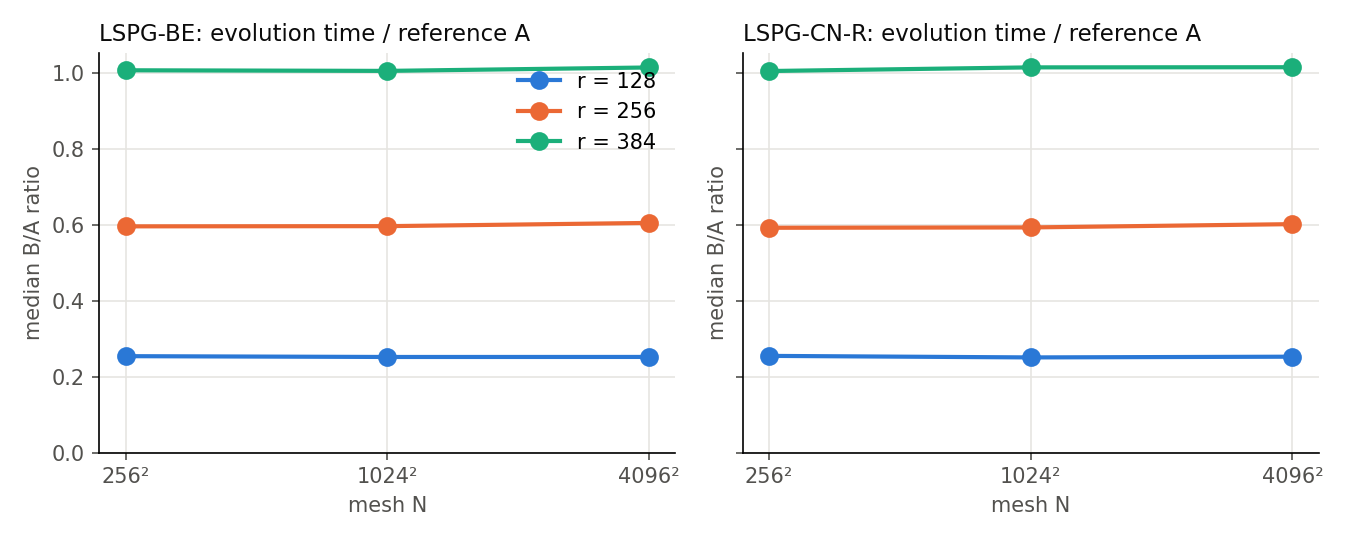
\includegraphics[width=0.48\linewidth]{figs/p1_solve_time_vs_mesh.png}\hfill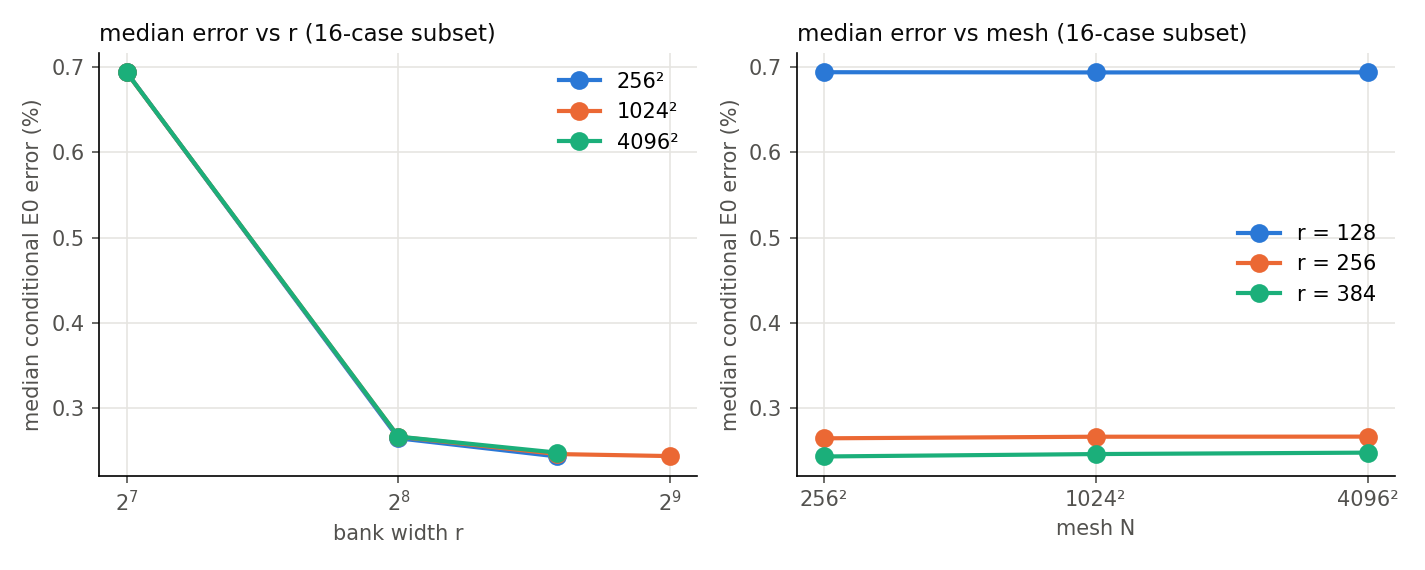
\includegraphics[width=0.48\linewidth]{figs/p1_error_cnr.png}\end{center}
\begin{center}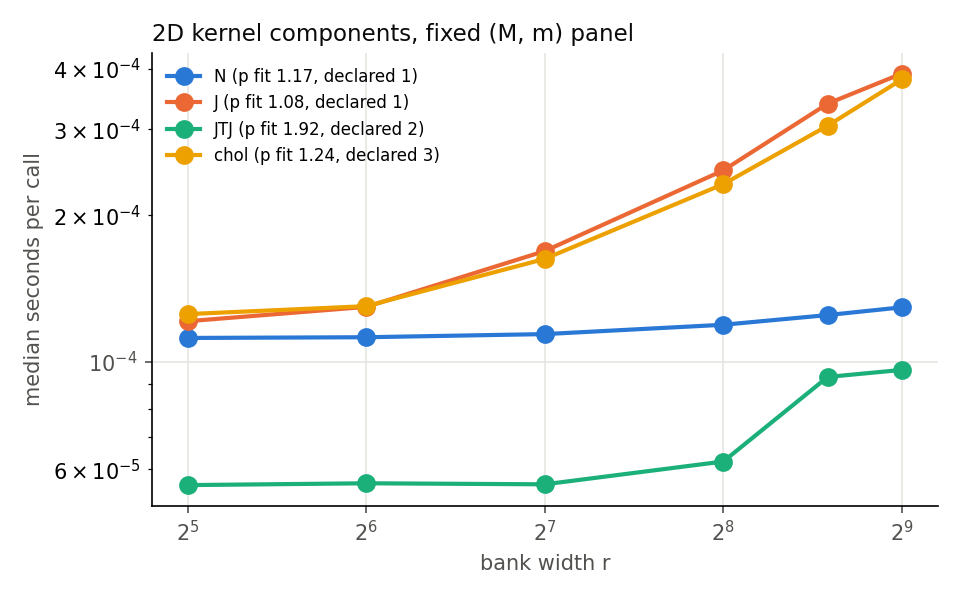
\includegraphics[width=0.48\linewidth]{figs/p1_kernel2d.png}\hfill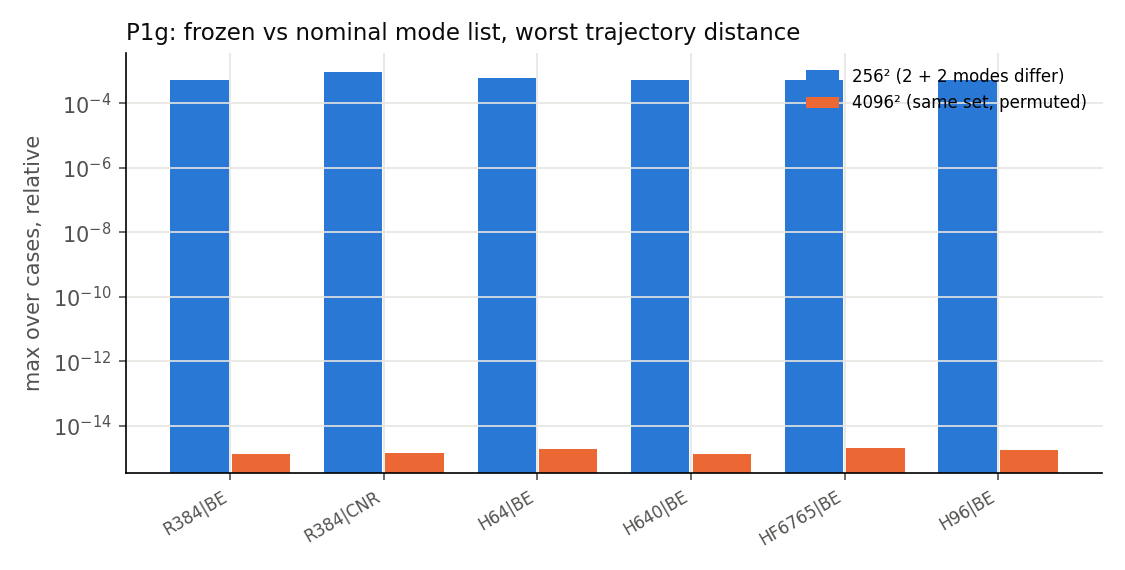
\includegraphics[width=0.48\linewidth]{figs/p1_p1g.png}\end{center}

\subsection*{Corrections}
\retracted{The coordinator's restatement said the 2D mode lists also differ at $4096^2$; they do not (permutation only). The plan's ``1024$^2$ reused from combined'' was false for R256 (different rule); all 1024$^2$ runs were redone. In the quadrature slice, \texttt{gauss64} was registered as the failing 2D rule but passes both bars (the pre-data expectation was wrong); in 3D \texttt{lat8192} fails (4.2e-3 > 2.5e-4). The first smoke acceptance failed 5 checks, all defects in the checks themselves. The component-sum control was demoted to a diagnostic (deviation from AM-5, disclosed).}
